\documentclass{standalone}
\usepackage{tikz}
\usetikzlibrary{calc}
\begin{document}
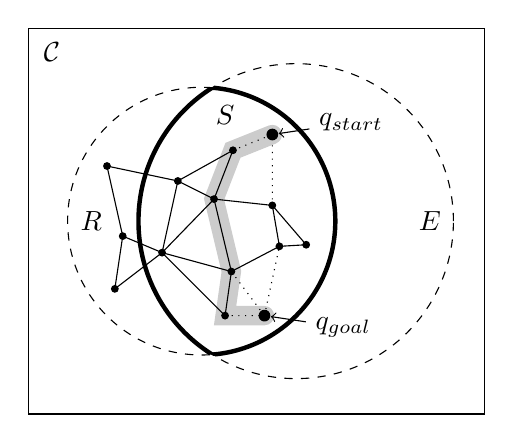
\begin{tikzpicture}

\draw (0,0) rectangle (5.8,4.9);

\coordinate (r) at (2.2,2.45);
\coordinate (e) at (3.4,2.45);

\def\circler{(r) circle (1.7)}
\def\circlee{(e) circle (2.0)}

% XnY
\begin{scope}
   \clip \circler;
   %\fill[pattern=horizontal lines] \circley;
   \draw[ultra thick] \circlee;
\end{scope}
\begin{scope}
   \clip \circlee;
   \draw[ultra thick] \circler;
\end{scope}

\draw[dashed] \circler;
\draw[dashed] \circlee;

\node (clab) at (0.3,4.6) {$\mathcal{C}$};
\node (rlab) at ($ (r) + (-1.4,0) $) {$R$};
\node (elab) at ($ (e) + ( 1.7,0) $) {$E$};
\node (flab) at (2.5,3.8) {$S$};

\coordinate (v01) at ($ (r) + (-1.20, 0.70) $);
\coordinate (v02) at ($ (r) + (-1.10,-0.86) $);
\coordinate (v03) at ($ (r) + (-1.00,-0.19) $);
\coordinate (v04) at ($ (r) + (-0.50,-0.40) $);
\coordinate (v05) at ($ (r) + (-0.30, 0.51) $);
\coordinate (v07) at ($ (r) + ( 0.30,-1.20) $);
\coordinate (v08) at ($ (r) + ( 0.16, 0.28) $);
\coordinate (v09) at ($ (r) + ( 0.38,-0.64) $);
\coordinate (v06) at ($ (r) + ( 0.40, 0.90) $);
\coordinate (v10) at ($ (r) + ( 0.90, 0.20) $);
\coordinate (v11) at ($ (r) + ( 0.99,-0.32) $);
\coordinate (v12) at ($ (r) + ( 1.33,-0.30) $);
\coordinate (p1) at ($ (r) + (0.9, 1.1) $);
\coordinate (p2) at ($ (r) + (0.8,-1.2) $);

\draw[color=black!20,line width=7,line cap=round]
  (p2) -- (v07) -- (v09) -- (v08) -- (v06) -- (p1);

\node[circle,fill=black,inner sep=1.0] at (v01) {};
\node[circle,fill=black,inner sep=1.0] at (v02) {};
\node[circle,fill=black,inner sep=1.0] at (v03) {};
\node[circle,fill=black,inner sep=1.0] at (v04) {};
\node[circle,fill=black,inner sep=1.0] at (v05) {};
\node[circle,fill=black,inner sep=1.0] at (v07) {};
\node[circle,fill=black,inner sep=1.0] at (v08) {};
\node[circle,fill=black,inner sep=1.0] at (v09) {};
\node[circle,fill=black,inner sep=1.0] at (v06) {};
\node[circle,fill=black,inner sep=1.0] at (v10) {};
\node[circle,fill=black,inner sep=1.0] at (v11) {};
\node[circle,fill=black,inner sep=1.0] at (v12) {};

\draw (v01) -- (v03) -- (v02) -- (v04) -- (v03);
\draw (v01) -- (v05) -- (v04) -- (v07) -- (v09) -- (v04);
\draw (v04) -- (v08) -- (v05) -- (v06) -- (v08) -- (v10);
\draw (v08) -- (v09) -- (v11) -- (v10);
\draw (v11) -- (v12) -- (v10);

\node[circle,fill=black,inner sep=1.5] (p1node) at (p1) {};
\node[circle,fill=black,inner sep=1.5] (p2node) at (p2) {};
\draw[color=black,dotted] (v06) -- (p1) -- (v10);
\draw[color=black,dotted] (v07) -- (p2) -- (v09);
\draw[color=black,dotted] (p2) -- (v11);

\node (p1lab) at (4.1,3.7) {$q_{start}$};
\node (p2lab) at (4.0,1.1) {$q_{goal}$};
\draw[->] (p1lab) -- (p1node);
\draw[->] (p2lab) -- (p2node);

\end{tikzpicture}%
\end{document}
